\section{交流电路}

\subsection{正弦交流电路的基本概念}

电流瞬时表达式:

\[
    i=I_m\sin(\omega t+\psi)
\]

其中,$I_m$为电流的最大值,$\omega$为角频率,$\psi$为初相位
或相位角。\\
波形图如下

\begin{tikzpicture}
    %\draw[very thin,color=gray] (-0.1,-1.1) grid (3.9,8.1);
    \draw[->,thick] (-0.5,0) -- (8,0) node[right] {$t$};
    \draw[->,thick] (0,-1.5) -- (0,2.5) node[above] {$i$};
    
    \draw[domain=-1:7,smooth] plot(\x,{2*sin(\x r + 30)});

\end{tikzpicture}



\

周期,频率

\[
    \omega=\frac{2\pi}{T}=2\pi f,~ f=\frac{1}{T}    
\]

最大值和有效值

\[
    U = \frac{U_m}{\sqrt{2}} ,~ 
    E = \frac{E_m}{\sqrt{2}} ,~
    I=\frac{I_m}{\sqrt{2}}
\]

\

$(\omega t + \psi)$称为相位,或相位角,$\psi$称为初相位。

任意两正弦量的相位差:$\varphi = \phi_2 - \phi_1$。

\large{\textbf{相量表示法}}

\normalsize
表示正弦交流电在复平面中处于起始位置的固定矢量称为正弦交流
电的相量。
\underline{
区分最大值相量和有效值相量
}

复平面的矢量可用复数表示,矢量$\overline{OP}$的表示方法如下:
\[
    \overline{OP}=a+jb = c(\cos \psi + j\sin \psi ) = ce^{j\psi}=c\phase{\psi}
\]

为避免符号混淆,在代表交流电的符号上加上一点,以示区别。$\dot{I},\dot{U}$

\large 注意事项
\normalsize
\begin{enumerate}
    \item 相量不等于正弦交流电
    \item 只有正弦交流电才能用相量表示
    \item 只有同频率的
    正弦交流电才能进行相量运算
\end{enumerate}

\subsection{单一参数交流电路}

\begin{center}
    \textbf{单一参数交流电路的主要结论}
\end{center}

\begin{table}[!ht]
    \resizebox{\textwidth}{!}{%
    \begin{tabular}{|cc|c|c|c|}
    \hline
    \multicolumn{2}{|c|}{项目} & 电阻 & 电容 & 电感 \\ \hline
    \multicolumn{2}{|c|}{电阻或阻抗} & $R$ & $X_C=\frac{1}{2\pi fC}$ & $X_L=2\pi fL$ \\ \hline
    \multicolumn{1}{|c|}{\multirow{4}{*}{电压与电流的关系}} & 频率 & 相图 & 相同 & 相同 \\ \cline{2-5} 
    \multicolumn{1}{|c|}{} & 相位 & 相同 & $u$ 滞后$i$$90^\circ$ & $u$ 超前$i$$90^\circ$ \\ \cline{2-5} 
    \multicolumn{1}{|c|}{} & 有效值 & $U=RI$ & $U=X_CI$ & $U=X_LI$ \\ \cline{2-5} 
    \multicolumn{1}{|c|}{} & 相量式 & $\dot{U}=R\dot{I}$ & $\dot{U}=-jX_C\dot{I}$ & $\dot{U}=jX_L\dot{I}$ \\ \hline
    \multicolumn{1}{|c|}{\multirow{2}{*}{功率}} & 有功功率 & $P=UI=R^2I=\frac{U^2}{R}$ & 0 & 0 \\ \cline{2-5} 
    \multicolumn{1}{|c|}{} & 无功功率 & 0 & $Q=UI=X_CI^2=\frac{U^2}{X_C}$ & $Q=UI=X_LI^2=\frac{U^2}{X_L}$ \\ \hline
    \end{tabular}%
    }
\end{table}

\subsection{串联和并联交流电路}

\subsubsection{串联交流电路}

\begin{center}
    \begin{circuitikz}[american voltages]
        \draw
        (0,0) to [short, o-] (1,0)
        to [american inductor, l=$L$] (5,0) 
        (0,0) to [open, v^>=$u$] (0,4) 
        to [short, o- ,i=$i$] (1,4) 
        to [R, l=$R$] (5,4)
        %to [L, l=$L_{\sigma}$] (5,4) 
        %to [short] (5,3) 
        to [capacitor, l_=$C$] (5,0);
    \end{circuitikz}
\end{center}

电抗 $X=X_L-X_C$
阻抗 
\[
    Z=R+jX
\]

显然阻抗不是相量,只是一般复数。同样可以写出四种形式:
\[
    Z=R+jX= \left\lvert Z \right\rvert (\cos \varphi + j\sin \varphi ) = \left\lvert Z \right\rvert \phase{\varphi} = \left\lvert Z \right\rvert e^{j\varphi}
\]

其中$\left\lvert Z \right\rvert$称为阻抗的模,
$\varphi$称为阻抗角。有下式成立:
\[
    \left\lvert Z \right\rvert = \sqrt{R^2+X^2},~ \varphi = \arctan \frac{X}{R} = \arccos \frac{R}{\left\lvert Z \right\rvert} = \arcsin \frac{X}{\left\lvert Z \right\rvert}
\]

电压和电流的关系:

\begin{itemize}
    \item 有效值:$U=\left\lvert Z \right\rvert I$
    \item 相量式:$\dot{U}=Z\dot{I}$
    \item 相位关系:$\varphi = \psi _u - \psi _i $
\end{itemize}

\subsubsection{并联交流电路}

解法有三种:
\begin{itemize}
    \item 先求支路电流再求总电流
     \[\dot{I}=\sum \dot{I_i}=\sum \frac{\dot{U}}{Z_i}\]
    \item 先求并联等效阻抗再求总电流 
    \[\dot{I}=\frac{\dot{U}}{Z} \]
    其中 
    \[\frac{1}{Z}=\sum \frac{1}{Z_i}\]
    \item 画出向量图,由几何关系求总电流
\end{itemize}


\subsection{交流电路的功率和功率因数}


\begin{wrapfigure}{right}{65mm}
    \centering
    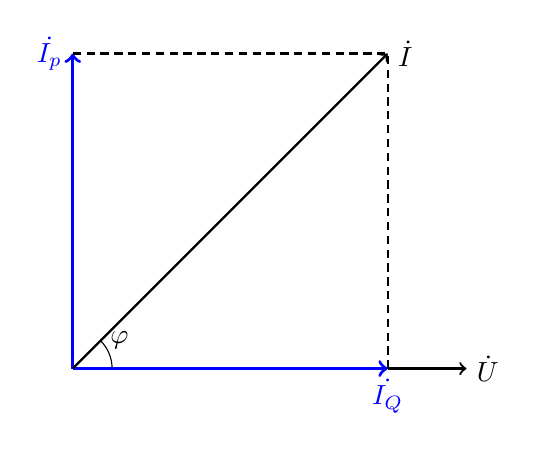
\begin{tikzpicture}
        %\draw[very thin,color=gray] (-0.1,-1.1) grid (3.9,8.1);
        \draw[->,very thick, color=blue] (0,0) -- (4,0) node[below] {$\dot{I_Q}$};
        \draw[->,very thick, color=blue] (0,0) -- (0,4) node[left] {$\dot{I_p}$};
        \draw[->,thick] (0,0) -- (4,4) node[right] {$\dot{I}$};
        \draw[densely dashed,thick] (4,0) to (4,4);
        \draw[densely dashed,thick] (0,4) to (4,4);
        \draw[->,thick] (4,0) to (5,0) node[right] {$\dot{U}$};
        \draw (0.5,0) arc (0:45:0.5) node[right] {$\varphi$};
        %\draw[domain=-1:7,smooth] plot(\x,{2*sin(\x r + 30)});
    \end{tikzpicture}   
\end{wrapfigure}
当电流与电压相位不同时,则电流可分解成两个分量,一个与电压同相位,
一个与电压相位相差$90^\circ$。前者为有功分量,后者为无功分量。如图所示.

显然
\[
    I_P=Icos\varphi,~ I_Q=Isin\varphi
\]

有功功率,无功功率和视在功率分别为

\[
    P=UI_P=UIcos\varphi,~ Q=UI_Q=UIsin\varphi,~ S=UI
\]

其单位分别为瓦$\text{W}$,乏$\text{var}$,伏安$\text{V}\cdot \text{A}$.
三种功率之间的关系为

\[
    S^2=P^2+Q^2
\]
\[
    P=S\cos\varphi 
\]
\[
    Q=S\sin\varphi 
\]

总功率与各部分功率之间的关系为

\[
    P=\sum P_i,~ Q=\sum Q_i,~ S \ne \sum S_i
\]

\textbf{在交流电路总,有用功率与视载功率的比值
用$\lambda$来表示,称为电路的功率因数。}

\[
    \lambda = \frac{P}{S} = \cos \varphi
\]
功率因数过大引起的问题:
\begin{itemize}
    \item 降低供电设备的利用率
    \item 增加供电设备和输电线路的功率损耗
\end{itemize}
并联电容提高感性电路的功率因数的电容求解方法:

\begin{example}
    有一感性负载接到交流电上频率为$f$,电压为$U$,功
    率因数为$\lambda_L$,消耗有用功为$P$,若要将功率因数提高到$\lambda$求并联电容$C$的大小。
    \begin{description}
        \item[解法一] 通过无功功率的变化\\
        未并联电容时,有功率因数为$\lambda_L$,则
        \[
            \varphi_L =\arccos \lambda_L
        \]
        \[
        S_L = \frac{P}{\cos \lambda_L}    
        \]
        \[
            Q_L = S_L\sin \varphi_L
        \]
        并入电容后,有功率因数为$\lambda$,则
        \[
            \varphi = \arccos \lambda
        \]
        \[
            S = \frac{P}{\cos \lambda}
        \]
        \[
            Q = S\sin \varphi
        \]
        减少的无功功率是由并联的电容提供的,故电容的无功功率绝对值为
        \[
            \left\lvert Q_C\right\rvert = \left\lvert Q - Q_L \right\rvert
        \]
        电容中的电流为
        \[
            I_C = \frac{\left\lvert Q_C\right\rvert}{U}
        \]
        即可计算出需要的容抗和电容
        \[
            X_C = \frac{U}{I_C},~ C = \frac{1}{2\pi f X_C}  
        \]            
        \item[解法二] 通过电流无功分量的变化\\
        未并联电容时
        \[
            I_L = \frac{P}{U\cos \varphi _L}
        \]
        \[
            \varphi_L = \arccos \lambda_L
        \]
        电流的无功分量为
        \[
            I_{QL} = I_L \sin \varphi_L
        \]
        并入电容后,有功率因数为$\lambda$,则
        \[
            \varphi = \arccos \lambda
        \]
        \[
            I = \frac{P}{U\cos \varphi}
        \]
        电流的无功分量为
        \[
            I_Q = I \sin \varphi
        \]
        电容中的电流为
        \[
            I_C = I_{QL}-I_Q =I_{L}\sin \varphi_L - I \sin \varphi
        \]
        后续步骤同解法一
        \item[解法三]直接带入公式\\
        由上述两种解法可推导出并联电容的公式为

        \[
            C = \frac{P}{2\pi f U^2}(\tan \varphi_L - \tan \varphi)  
        \]
        
    \end{description}
\end{example}

\subsection{电路中的谐振}
使用交流电流中当电路中的电感和电容的电抗相等时,电路中的
电流和电压的幅值达到最大值,这种现象称为谐振。\\
品质因数$Q$值是描述谐振现象的一个重要参数。
\[
    Q_f = \frac{\left\lvert Q_L ~ \text{or} ~ Q_C\right\rvert }{P}
\]

\noindent 串联谐振特点:
\begin{itemize}
    \item $Q_L$ 与 $Q_C$ 相互补偿,$Q=0,S=P,\lambda =1$
    \item $X_L$ 与 $X_C$ 数值相等,$X=0$,$Z=R$最小,$I=\frac{U}{R}$最大
    \item $U_L$ 与 $U_C$ 相互抵消,$U_X=0,U=U_R$
    \item $Q_f=\frac{1}{R}\sqrt{\frac{L}{C}}$
\end{itemize}

\noindent 并联谐振特点:
\begin{itemize}
    \item $Q_L$ 与 $Q_C$ 相互补偿,$Q=0,S=P,\lambda =1$
    \item $X_L$ 与 $X_C$ 数值相等,$X=0$,$Z_{LC}=\frac{-\text{j}X_C\cdot \text{j}X_C}{\text{j}X_C- \text{j}X_C}\rightarrow \infty$,$Z=R$最大
    \item $I_L$ 与 $I_C$ 相互抵消,$I_X=0,I=I_R$
    \item $Q_f=\frac{1}{R}\sqrt{\frac{C}{L}}$
\end{itemize}
